\documentclass[aspectratio=169]{beamer}
\usetheme{Madrid}
\usecolortheme{default}

\usepackage[utf8]{inputenc}
\usepackage[T5]{fontenc}
\usepackage[vietnamese]{babel}
\usepackage{helvet}
\renewcommand{\familydefault}{\sfdefault}
\usepackage{tikz}
\usepackage{graphicx}
\usepackage{booktabs}
\usepackage{xcolor}
\usepackage{array}
\usepackage{multirow}
\usepackage{colortbl}
\usepackage[most]{tcolorbox}
\usepackage{listings}
\usetikzlibrary{shapes.geometric, arrows.meta, positioning, calc, fit, backgrounds, shadows.blur}

\definecolor{primary}{RGB}{37, 99, 235}
\definecolor{secondary}{RGB}{16, 185, 129}
\definecolor{accent}{RGB}{245, 158, 11}
\definecolor{dark}{RGB}{30, 41, 59}
\definecolor{best}{RGB}{34, 197, 94}
\definecolor{danger}{RGB}{239, 68, 68}
\definecolor{lightgray}{RGB}{243, 244, 246}

\tikzset{
    box/.style={rectangle, rounded corners=4pt, draw=dark, thick, align=center, font=\small\bfseries, inner sep=6pt},
    component/.style={box, fill=white, drop shadow={opacity=0.12, shadow xshift=1pt, shadow yshift=-1pt}},
    db/.style={cylinder, shape border rotate=90, aspect=0.28, draw=dark, thick, align=center, font=\scriptsize\bfseries, inner sep=4pt},
    queue/.style={rectangle, rounded corners=8pt, draw=accent, thick, fill=accent!12, align=center, font=\scriptsize\bfseries, inner sep=5pt},
    arr/.style={-{Stealth[length=2mm]}, thick, dark},
    dasharr/.style={-{Stealth[length=2mm]}, dashed, thick, dark}
}

\setbeamertemplate{navigation symbols}{}
\setbeamercolor{structure}{fg=primary}
\setbeamercolor{frametitle}{bg=primary, fg=white}
\setbeamercolor{title}{bg=primary, fg=white}
\setbeamercolor{item}{fg=accent}
\setbeamertemplate{itemize item}{\color{accent}$\blacktriangleright$}
\setbeamertemplate{footline}[frame number]
\setbeamersize{text margin left=0.55cm,text margin right=0.55cm}

\newtcolorbox{claimbox}[2][]{colback=#2!10, colframe=#2, boxrule=0.9pt, arc=3pt, left=5pt, right=5pt, top=4pt, bottom=4pt, #1}

\title[URL Shortener Microservices]{\textbf{URL Shortener Microservices}}
\subtitle{Thiết kế, triển khai và vận hành hệ thống rút gọn URL theo kiến trúc Microservices}
\author{Đồ án môn học SE361.Q21 \textemdash{} Phát triển phần mềm theo kiến trúc Microservices}
\institute{University of Information Technology \textemdash{} VNU-HCM}
\date{2026}

\begin{document}

\begin{frame}
    \titlepage
\end{frame}

\begin{frame}{Thông điệp chính}
    \begin{columns}[T,onlytextwidth]
        \begin{column}{0.33\textwidth}
            \begin{claimbox}{primary}
                \centering\large\textbf{Không phải app CRUD}\par
                \vspace{0.15cm}
                \small Một use case đọc rất nhiều: redirect phải nhanh, ổn định, không phụ thuộc analytics.
            \end{claimbox}
        \end{column}
        \begin{column}{0.33\textwidth}
            \begin{claimbox}{secondary}
                \centering\large\textbf{Microservice đúng nghĩa}\par
                \vspace{0.15cm}
                \small Bounded context, database riêng, API Gateway, HTTP sync và RabbitMQ async.
            \end{claimbox}
        \end{column}
        \begin{column}{0.33\textwidth}
            \begin{claimbox}{accent}
                \centering\large\textbf{Có vận hành}\par
                \vspace{0.15cm}
                \small Docker Compose, healthcheck, Prometheus, Grafana, smoke test, k6 load test.
            \end{claimbox}
        \end{column}
    \end{columns}

    \vspace{0.55cm}
    \begin{center}
        \begin{claimbox}[width=0.86\textwidth, halign=center]{best}
            \textbf{Idea bảo vệ:} hệ thống nhỏ về nghiệp vụ, nhưng đầy đủ các vấn đề thật của microservices: chia domain, dữ liệu phân tán, messaging, cache, resilience, observability và kiểm thử.
        \end{claimbox}
    \end{center}
\end{frame}

\begin{frame}{Bám sát mục tiêu môn SE361}
    \begin{columns}[T,onlytextwidth]
        \begin{column}{0.48\textwidth}
            \textbf{Đề cương nhắm tới}
            \vspace{0.2cm}
            \begin{tikzpicture}[scale=0.72, transform shape]
                \node[component, fill=primary!12, minimum width=4.8cm] at (0,2.4) {DDD \& Bounded Context};
                \node[component, fill=secondary!12, minimum width=4.8cm] at (0,1.3) {REST + Async Messaging};
                \node[component, fill=accent!15, minimum width=4.8cm] at (0,0.2) {Database per Service};
                \node[component, fill=danger!10, minimum width=4.8cm] at (0,-0.9) {Security + Resilience};
                \node[component, fill=best!12, minimum width=4.8cm] at (0,-2.0) {Docker + Monitoring + Testing};
            \end{tikzpicture}
        \end{column}
        \begin{column}{0.48\textwidth}
            \textbf{Dự án đã hiện thực}
            \vspace{0.2cm}
            \begin{claimbox}{primary}
                \small 5 binary Go độc lập: gateway, user, url, analytics, notification.
            \end{claimbox}
            \begin{claimbox}{secondary}
                \small HTTP/JSON qua gateway; RabbitMQ topic exchange cho click, created, deleted, milestone.
            \end{claimbox}
            \begin{claimbox}{accent}
                \small 4 PostgreSQL database riêng; Redis chỉ làm cache và rate-limit store.
            \end{claimbox}
            \begin{claimbox}{best}
                \small Prometheus/Grafana, circuit breaker, k6 script, smoke/e2e scripts.
            \end{claimbox}
        \end{column}
    \end{columns}
\end{frame}

\begin{frame}{Bài toán: URL Shortener không đơn giản như nhìn thấy}
    \begin{columns}[T,onlytextwidth]
        \begin{column}{0.47\textwidth}
            \begin{claimbox}{danger}
                \textbf{Nếu làm kiểu monolith đơn giản}
                \begin{itemize}\tiny
                    \item Redirect, analytics, notification dính vào cùng request path.
                    \item Analytics lỗi có thể kéo chậm redirect.
                    \item Scale phải scale cả khối dù chỉ redirect nóng.
                    \item DB chung dễ sinh join chéo và coupling schema.
                \end{itemize}
            \end{claimbox}
        \end{column}
        \begin{column}{0.47\textwidth}
            \begin{claimbox}{best}
                \textbf{Cách tiếp cận microservices}
                \begin{itemize}\small
                    \item Redirect là hot path, ưu tiên cache và latency.
                    \item Analytics/notification xử lý bất đồng bộ qua event.
                    \item Mỗi service sở hữu dữ liệu của mình.
                    \item Gateway bảo vệ hệ thống bằng auth, rate limit, circuit breaker.
                \end{itemize}
            \end{claimbox}
        \end{column}
    \end{columns}
    \vspace{0.25cm}
    \begin{center}
        \begin{claimbox}[width=0.86\textwidth, halign=center]{primary}
            \textbf{Mục tiêu thiết kế:} redirect nhanh khi phụ trợ lỗi một phần, nhưng vẫn thu thập click và gửi thông báo bằng event.
        \end{claimbox}
    \end{center}
\end{frame}

\begin{frame}{Tách Bounded Context}
    \begin{center}
    \begin{tikzpicture}[scale=0.76, transform shape]
        \node[component, fill=primary!12, minimum width=2.8cm, minimum height=1cm] (gw) at (0,2.2) {API Gateway};
        \node[component, fill=secondary!12, minimum width=2.8cm, minimum height=1cm] (user) at (-5,0.3) {User Service\scriptsize Auth, JWT};
        \node[component, fill=best!12, minimum width=2.8cm, minimum height=1cm] (url) at (-1.7,0.3) {URL Service\scriptsize Shorten, Redirect};
        \node[component, fill=accent!15, minimum width=2.8cm, minimum height=1cm] (ana) at (1.7,0.3) {Analytics\scriptsize Click stats};
        \node[component, fill=danger!10, minimum width=2.8cm, minimum height=1cm] (noti) at (5,0.3) {Notification\scriptsize Events, email log};

        \node[db, fill=secondary!10, minimum width=1.4cm] (userdb) at (-5,-1.7) {user\_db};
        \node[db, fill=best!10, minimum width=1.4cm] (urldb) at (-1.7,-1.7) {url\_db};
        \node[db, fill=accent!10, minimum width=1.4cm] (anadb) at (1.7,-1.7) {analytics\_db};
        \node[db, fill=danger!8, minimum width=1.4cm] (notidb) at (5,-1.7) {notification\_db};

        \draw[arr] (gw) -- (user);
        \draw[arr] (gw) -- (url);
        \draw[arr] (gw) -- (ana);
        \draw[arr] (gw) -- (noti);
        \draw[arr] (user) -- (userdb);
        \draw[arr] (url) -- (urldb);
        \draw[arr] (ana) -- (anadb);
        \draw[arr] (noti) -- (notidb);
    \end{tikzpicture}
    \end{center}
    \vspace{-0.1cm}
    \begin{claimbox}{primary}
        \small \textbf{Điểm cần nhấn mạnh:} monorepo chỉ là cách tổ chức source code; ranh giới runtime là binary, container, API và database riêng.
    \end{claimbox}
\end{frame}

\begin{frame}{Kiến trúc tổng quan}
    \begin{center}
    \begin{tikzpicture}[scale=0.62, transform shape]
        \node[circle, draw=dark, fill=lightgray, minimum size=0.9cm, font=\small\bfseries] (client) at (-7,1.7) {Client};
        \node[component, fill=primary!14, minimum width=2.5cm] (gw) at (-4,1.7) {Gateway\scriptsize :8080};
        \node[component, fill=secondary!12, minimum width=2.3cm] (user) at (-0.5,3.2) {user-service\scriptsize :8083};
        \node[component, fill=best!12, minimum width=2.3cm] (url) at (-0.5,1.7) {url-service\scriptsize :8081};
        \node[component, fill=accent!14, minimum width=2.3cm] (ana) at (-0.5,0.2) {analytics\scriptsize :8082};
        \node[component, fill=danger!10, minimum width=2.3cm] (noti) at (-0.5,-1.3) {notification\scriptsize :8084};

        \node[db, fill=secondary!10] (userdb) at (2.4,3.2) {Postgres};
        \node[db, fill=best!10] (urldb) at (2.4,1.7) {Postgres};
        \node[db, fill=accent!10] (anadb) at (2.4,0.2) {Postgres};
        \node[db, fill=danger!8] (notidb) at (2.4,-1.3) {Postgres};
        \node[component, fill=best!20, minimum width=1.7cm] (redis) at (2.4,-2.8) {Redis};
        \node[queue, minimum width=2.4cm] (mq) at (5.5,0.4) {RabbitMQ\scriptsize topic exchange};
        \node[component, fill=primary!8, minimum width=2.2cm] (prom) at (-4,-1.4) {Prometheus\scriptsize /metrics};
        \node[component, fill=accent!10, minimum width=2.2cm] (graf) at (-4,-2.8) {Grafana\scriptsize dashboard};

        \draw[arr] (client) -- (gw);
        \draw[arr] (gw) -- (user); \draw[arr] (gw) -- (url); \draw[arr] (gw) -- (ana); \draw[arr] (gw) -- (noti);
        \draw[arr] (user) -- (userdb); \draw[arr] (url) -- (urldb); \draw[arr] (ana) -- (anadb); \draw[arr] (noti) -- (notidb);
        \draw[arr] (url) -- (redis);
        \draw[arr] (gw) -- (redis);
        \draw[dasharr] (url) -- node[above, font=\tiny] {created/clicked/deleted} (mq);
        \draw[dasharr] (mq) -- (ana);
        \draw[dasharr] (mq) -- (noti);
        \draw[dasharr] (ana) -- node[right, font=\tiny] {milestone} (mq);
        \draw[arr] (prom) -- (graf);
        \draw[dasharr] (gw) -- (prom);
    \end{tikzpicture}
    \end{center}
\end{frame}

\begin{frame}{API Gateway: cửa vào duy nhất}
    \begin{columns}[T,onlytextwidth]
        \begin{column}{0.50\textwidth}
            \begin{claimbox}{primary}
                \textbf{Gateway làm ở edge}
                \begin{itemize}\small
                    \item Reverse proxy route theo path.
                    \item JWT validation cho route private.
                    \item Rate limit theo IP bằng Redis.
                    \item Circuit breaker từng upstream.
                    \item Gắn \texttt{X-Correlation-ID}.
                    \item Expose \texttt{/metrics} cho Prometheus.
                \end{itemize}
            \end{claimbox}
        \end{column}
        \begin{column}{0.46\textwidth}
            \begin{tikzpicture}[scale=0.74, transform shape]
                \node[component, fill=lightgray, minimum width=4.5cm] (req) at (0,2.5) {Request};
                \node[component, fill=primary!12, minimum width=4.5cm] (auth) at (0,1.45) {Auth middleware};
                \node[component, fill=accent!14, minimum width=4.5cm] (rl) at (0,0.4) {Rate limit};
                \node[component, fill=danger!10, minimum width=4.5cm] (cb) at (0,-0.65) {Circuit breaker};
                \node[component, fill=best!12, minimum width=4.5cm] (proxy) at (0,-1.7) {Proxy to service};
                \draw[arr] (req)--(auth); \draw[arr] (auth)--(rl); \draw[arr] (rl)--(cb); \draw[arr] (cb)--(proxy);
            \end{tikzpicture}
        \end{column}
    \end{columns}
\end{frame}

\begin{frame}{REST API surface}
    \scriptsize
    \begin{center}
    \begin{tabular}{>{\bfseries}p{0.22\textwidth}p{0.34\textwidth}p{0.34\textwidth}}
        \toprule
        Nhóm & Gateway endpoint & Trách nhiệm service \\
        \midrule
        Auth & \texttt{POST /api/auth/register}, \texttt{POST /api/auth/login}, \texttt{GET /api/me} & Register, login, bcrypt, JWT, profile \\
        URL & \texttt{POST /api/shorten}, \texttt{GET /api/urls}, \texttt{DELETE /api/urls/\{code\}} & Short code, ownership, deactivate, outbox \\
        Redirect & \texttt{GET /r/\{code\}} & Redis cache, DB fallback, 301 redirect, click event \\
        Analytics & \texttt{GET /api/stats/\{code\}}, timeline & Total click, 24h, 7d, referer, time bucket \\
        Notification & \texttt{GET /api/notifications} & List notification theo user, cursor paging \\
        \bottomrule
    \end{tabular}
    \end{center}
    \vspace{0.35cm}
    \begin{claimbox}{secondary}
        \small \textbf{RESTful + pragmatic:} route public/private rõ, list API có cursor pagination, limit được clamp, body auth giới hạn 1MB.
    \end{claimbox}
\end{frame}

\begin{frame}{URL Service: hot path được tối ưu}
    \begin{columns}[T,onlytextwidth]
        \begin{column}{0.48\textwidth}
            \begin{claimbox}{best}
                \textbf{Shorten}
                \begin{itemize}\small
                    \item Validate URL chỉ nhận \texttt{http}/\texttt{https}.
                    \item Sinh base62 7 ký tự bằng \texttt{crypto/rand}.
                    \item Không gian mã: \texttt{62\^{}7} $\approx$ 3.5 nghìn tỷ.
                    \item Unique constraint + retry collision.
                    \item Ghi \texttt{url.created} vào outbox trong transaction.
                \end{itemize}
            \end{claimbox}
        \end{column}
        \begin{column}{0.48\textwidth}
            \begin{claimbox}{primary}
                \textbf{Redirect}
                \begin{itemize}\small
                    \item Redis read-through cache, timeout 50ms.
                    \item Redis lỗi/cache miss thì fallback PostgreSQL.
                    \item Check inactive/expired trả 410.
                    \item Hash IP, ghi user-agent/referer.
                    \item Click analytics đi qua event, không block bởi consumer.
                \end{itemize}
            \end{claimbox}
        \end{column}
    \end{columns}
\end{frame}

\begin{frame}{Redis: nhanh nhưng không phải source of truth}
    \begin{center}
    \begin{tikzpicture}[scale=0.75, transform shape]
        \node[component, fill=lightgray, minimum width=2.2cm] (req) at (-5,1.2) {GET /r/code};
        \node[component, fill=best!16, minimum width=2.2cm] (redis) at (-1.8,1.2) {Redis GET\scriptsize 50ms timeout};
        \node[component, fill=secondary!15, minimum width=2.2cm] (hit) at (1.5,2.2) {Cache hit\scriptsize redirect ngay};
        \node[db, fill=primary!10, minimum width=1.7cm] (db) at (1.5,0.2) {PostgreSQL};
        \node[component, fill=accent!12, minimum width=2.3cm] (set) at (4.8,0.2) {Background\scriptsize cache set};
        \node[component, fill=best!20, minimum width=2.2cm] (redir) at (4.8,2.2) {301 Redirect};

        \draw[arr] (req)--(redis);
        \draw[arr] (redis)--node[above, font=\tiny]{hit}(hit);
        \draw[arr] (hit)--(redir);
        \draw[arr] (redis)--node[below, font=\tiny]{miss/error}(db);
        \draw[arr] (db)--(set);
        \draw[arr] (db.east)--++(1.2,0)--++(0,2.0)--(redir.west);
    \end{tikzpicture}
    \end{center}
    \begin{claimbox}{accent}
        \small \textbf{Câu trả lời khi bị hỏi:} Redis mất thì hệ thống chậm hơn nhưng không mất dữ liệu; PostgreSQL vẫn là nguồn dữ liệu đúng duy nhất.
    \end{claimbox}
\end{frame}

\begin{frame}{Event-driven: analytics và notification không kéo chậm redirect}
    \begin{center}
    \begin{tikzpicture}[scale=0.72, transform shape]
        \node[component, fill=best!12, minimum width=2.4cm] (url) at (-5,1.1) {url-service};
        \node[db, fill=best!10] (outbox) at (-2.6,1.1) {outbox};
        \node[queue, minimum width=2.8cm] (mq) at (0.4,1.1) {RabbitMQ\scriptsize url-shortener};
        \node[queue, minimum width=2.4cm, fill=primary!10, draw=primary] (q1) at (3.4,2.2) {analytics.clicks};
        \node[queue, minimum width=2.4cm, fill=danger!8, draw=danger] (q2) at (3.4,0.0) {notifications.events};
        \node[component, fill=accent!14, minimum width=2.2cm] (ana) at (6.2,2.2) {analytics-service};
        \node[component, fill=danger!10, minimum width=2.2cm] (noti) at (6.2,0.0) {notification-service};

        \draw[arr] (url)--node[above, font=\tiny]{same transaction}(outbox);
        \draw[arr] (outbox)--node[above, font=\tiny]{worker pool}(mq);
        \draw[arr] (mq)--node[above, font=\tiny]{url.clicked}(q1);
        \draw[arr] (mq)--node[below, font=\tiny]{created/deleted/milestone}(q2);
        \draw[arr] (q1)--(ana);
        \draw[arr] (q2)--(noti);
        \draw[dasharr] (ana.south)--++(0,-1.0)-| node[pos=0.25, below, font=\tiny]{milestone.reached}(mq.south);
    \end{tikzpicture}
    \end{center}
    \begin{claimbox}{secondary}
        \small Event payload chứa đủ dữ liệu để consumer xử lý, giảm gọi ngược service khác. Đây là trade-off denormalization có chủ đích để giảm coupling.
    \end{claimbox}
\end{frame}

\begin{frame}{Outbox Pattern: không để mất event khi broker lỗi}
    \begin{columns}[T,onlytextwidth]
        \begin{column}{0.47\textwidth}
            \begin{claimbox}{danger}
                \textbf{Nếu publish trực tiếp}
                \begin{itemize}\small
                    \item Ghi URL thành công.
                    \item RabbitMQ timeout đúng lúc publish.
                    \item DB có dữ liệu nhưng analytics không biết.
                    \item Dễ mất event, khó reconcile.
                \end{itemize}
            \end{claimbox}
        \end{column}
        \begin{column}{0.47\textwidth}
            \begin{claimbox}{best}
                \textbf{Cách dự án làm}
                \begin{itemize}\small
                    \item Ghi URL và event vào \texttt{outbox} cùng transaction.
                    \item Worker poll mỗi 2 giây, batch 50.
                    \item 3 worker goroutines.
                    \item \texttt{FOR UPDATE SKIP LOCKED} tránh đụng nhau.
                    \item Publish xong mới set \texttt{published\_at}.
                \end{itemize}
            \end{claimbox}
        \end{column}
    \end{columns}
\end{frame}

\begin{frame}{Analytics Service: xử lý đúng trước khi xử lý nhanh}
    \begin{columns}[T,onlytextwidth]
        \begin{column}{0.49\textwidth}
            \begin{claimbox}{accent}
                \textbf{Consumer behavior}
                \begin{itemize}\small
                    \item Consume \texttt{url.clicked} từ RabbitMQ.
                    \item Manual ack/nack.
                    \item QOS prefetch 1 để kiểm soát áp lực.
                    \item Invalid JSON hoặc thiếu event id thì ack và discard.
                    \item Deduplicate bằng bảng \texttt{processed\_events}.
                \end{itemize}
            \end{claimbox}
        \end{column}
        \begin{column}{0.47\textwidth}
            \begin{claimbox}{primary}
                \textbf{Stats API}
                \begin{itemize}\small
                    \item Total clicks.
                    \item Clicks last 24h và last 7d.
                    \item Top referers.
                    \item Timeline theo \texttt{day} hoặc \texttt{hour}.
                    \item Query song song bằng \texttt{errgroup}.
                    \item Milestone: 10, 100, 1000 clicks.
                \end{itemize}
            \end{claimbox}
        \end{column}
    \end{columns}
\end{frame}

\begin{frame}{Notification Service: side effect được cô lập}
    \begin{columns}[T,onlytextwidth]
        \begin{column}{0.45\textwidth}
            \begin{tikzpicture}[scale=0.74, transform shape]
                \node[queue, minimum width=4.2cm] (events) at (0,2.0) {url.created\quad url.deleted\quad milestone};
                \node[component, fill=danger!10, minimum width=4.2cm] (svc) at (0,0.7) {notification-service};
                \node[db, fill=danger!8, minimum width=1.6cm] (db) at (-1.3,-0.8) {notifications};
                \node[component, fill=lightgray, minimum width=1.8cm] (email) at (1.5,-0.8) {Mock email\scriptsize log};
                \draw[arr] (events)--(svc);
                \draw[arr] (svc)--(db);
                \draw[arr] (svc)--(email);
            \end{tikzpicture}
        \end{column}
        \begin{column}{0.51\textwidth}
            \begin{claimbox}{secondary}
                \textbf{Điểm nhỏ nhưng nên kể}
                \begin{itemize}\small
                    \item Consumer không làm URL Service chậm.
                    \item Notification lưu trạng thái \texttt{pending}, \texttt{sent}, \texttt{sent\_at}.
                    \item List notification theo user có cursor pagination.
                    \item Event \texttt{url.created} chứa email để tránh gọi ngược user-service.
                    \item Mock email giúp chứng minh flow side-effect mà không cần SMTP thật.
                \end{itemize}
            \end{claimbox}
        \end{column}
    \end{columns}
\end{frame}

\begin{frame}{Security: đủ lớp cần thiết cho đồ án}
    \begin{columns}[T,onlytextwidth]
        \begin{column}{0.33\textwidth}
            \begin{claimbox}{primary}
                \centering\textbf{Identity}\par\small
                Register/login, email unique, password tối thiểu 8 ký tự, bcrypt hash.
            \end{claimbox}
        \end{column}
        \begin{column}{0.33\textwidth}
            \begin{claimbox}{secondary}
                \centering\textbf{JWT}\par\small
                HS256, claims \texttt{sub/email/iss/iat/exp}, verify signing method HMAC.
            \end{claimbox}
        \end{column}
        \begin{column}{0.33\textwidth}
            \begin{claimbox}{accent}
                \centering\textbf{Data protection}\par\small
                Không lưu raw password, hash IP trước khi đưa vào analytics, ownership check khi delete URL.
            \end{claimbox}
        \end{column}
    \end{columns}
    \vspace{0.5cm}
    \begin{claimbox}{danger}
        \small \textbf{Nói thật khi bị hỏi production:} demo compose còn hard-code secrets, chưa TLS, chưa refresh token/revocation, chưa RBAC/OAuth2 đầy đủ. Đây là điểm mở rộng, không nên nói quá.
    \end{claimbox}
\end{frame}

\begin{frame}{Resilience: khi downstream chết, gateway không chết theo}
    \begin{center}
    \begin{tikzpicture}[scale=0.78, transform shape]
        \node[component, fill=best!12, minimum width=2.1cm] (closed) at (-4,1.2) {CLOSED\scriptsize gọi bình thường};
        \node[component, fill=danger!12, minimum width=2.1cm] (open) at (0,1.2) {OPEN\scriptsize trả 503 nhanh};
        \node[component, fill=accent!14, minimum width=2.1cm] (half) at (4,1.2) {HALF\_OPEN\scriptsize probe};
        \draw[arr] (closed)--node[above, font=\tiny]{5 lỗi / 10s}(open);
        \draw[arr] (open)--node[above, font=\tiny]{30s timeout}(half);
        \draw[arr] (half).. controls (2,-0.6) and (-2,-0.6) .. node[below, font=\tiny]{probe OK}(closed);
        \draw[arr, color=danger] (half).. controls (4.6,0.0) and (1.0,0.0) .. node[below, font=\tiny]{probe fail}(open);
    \end{tikzpicture}
    \end{center}
    \vspace{0.2cm}
    \begin{columns}[T,onlytextwidth]
        \begin{column}{0.48\textwidth}
            \begin{claimbox}{primary}
                \small \textbf{Circuit breaker:} giảm cascading failure, tránh request treo hàng loạt khi service chết.
            \end{claimbox}
        \end{column}
        \begin{column}{0.48\textwidth}
            \begin{claimbox}{accent}
                \small \textbf{Rate limit:} shorten 10 request/phút/IP, redirect 300 request/phút/IP; Redis lỗi thì fail-open.
            \end{claimbox}
        \end{column}
    \end{columns}
\end{frame}

\begin{frame}{Scalability: scale theo nút cổ chai, không scale cả cục}
    \begin{columns}[T,onlytextwidth]
        \begin{column}{0.48\textwidth}
            \begin{claimbox}{best}
                \textbf{Redirect đọc nhiều}
                \begin{itemize}\small
                    \item Cache Redis giảm query DB.
                    \item Gateway và url-service stateless ở tầng HTTP.
                    \item Có thể tăng replica cho gateway/url-service.
                    \item DB index theo \texttt{short\_code}.
                \end{itemize}
            \end{claimbox}
        \end{column}
        \begin{column}{0.48\textwidth}
            \begin{claimbox}{accent}
                \textbf{Async workload}
                \begin{itemize}\small
                    \item Analytics/notification tách khỏi request path.
                    \item Outbox worker pool 3 goroutines.
                    \item RabbitMQ durable queue hấp thụ spike.
                    \item Milestone có unique constraint chống phát nhiều lần.
                \end{itemize}
            \end{claimbox}
        \end{column}
    \end{columns}
    \vspace{0.35cm}
    \begin{claimbox}{primary}
        \small \textbf{Cẩn thận khi nói:} Docker Compose hiện demo một replica; thiết kế cho horizontal scaling nhưng chưa triển khai Kubernetes/service discovery động.
    \end{claimbox}
\end{frame}

\begin{frame}{Database per Service}
    \scriptsize
    \begin{center}
    \begin{tabular}{>{\bfseries}p{0.19\textwidth}p{0.25\textwidth}p{0.43\textwidth}}
        \toprule
        Service & Database & Bảng/ý nghĩa chính \\
        \midrule
        user-service & \texttt{user\_db} & \texttt{users}: email unique, password hash, created at \\
        url-service & \texttt{url\_db} & \texttt{urls}, \texttt{outbox}; index \texttt{short\_code}, \texttt{user\_id, created\_at} \\
        analytics & \texttt{analytics\_db} & \texttt{clicks}, \texttt{milestones}, \texttt{processed\_events} dedup \\
        notification & \texttt{notification\_db} & \texttt{notifications}: payload JSONB, status, sent at \\
        \bottomrule
    \end{tabular}
    \end{center}
    \vspace{0.3cm}
    \begin{claimbox}{secondary}
        \small \textbf{Luận điểm bảo vệ:} không cross-service join, không shared schema. Consistency giữa services đạt bằng event và eventual consistency.
    \end{claimbox}
\end{frame}

\begin{frame}{Observability: biết hệ thống đang sống hay đang gãy}
    \begin{columns}[T,onlytextwidth]
        \begin{column}{0.50\textwidth}
            \begin{claimbox}{primary}
                \textbf{Signals đã có}
                \begin{itemize}\small
                    \item Structured JSON logs bằng \texttt{slog}.
                    \item \texttt{X-Correlation-ID} xuyên gateway.
                    \item Gateway metrics Prometheus.
                    \item Grafana dashboard Circuit Breaker Monitor.
                    \item Health endpoint cho từng service.
                \end{itemize}
            \end{claimbox}
        \end{column}
        \begin{column}{0.46\textwidth}
            \begin{tikzpicture}[scale=0.72, transform shape]
                \node[component, fill=primary!12, minimum width=4cm] (gw) at (0,2.0) {gateway /metrics};
                \node[component, fill=secondary!12, minimum width=4cm] (prom) at (0,0.8) {Prometheus scrape 5s};
                \node[component, fill=accent!14, minimum width=4cm] (graf) at (0,-0.4) {Grafana dashboard};
                \node[component, fill=danger!10, minimum width=4cm] (ops) at (0,-1.6) {CB state, RPS, error rate};
                \draw[arr] (gw)--(prom); \draw[arr] (prom)--(graf); \draw[arr] (graf)--(ops);
            \end{tikzpicture}
        \end{column}
    \end{columns}
\end{frame}

\begin{frame}{Load testing: chứng minh chịu tải và circuit breaker}
    \begin{columns}[T,onlytextwidth]
        \begin{column}{0.47\textwidth}
            \begin{claimbox}{best}
                \textbf{k6 scenario}
                \begin{itemize}\small
                    \item Start stack: \texttt{docker compose up -d --build}.
                    \item Smoke test health bằng script.
                    \item k6 tự register user, login, shorten URL.
                    \item Load test endpoint nóng: \texttt{/r/\{shortCode\}}.
                    \item Target script hướng tới 10,000 req/s.
                \end{itemize}
            \end{claimbox}
        \end{column}
        \begin{column}{0.49\textwidth}
            \begin{claimbox}{danger}
                \textbf{Demo failure thật}
                \begin{itemize}\small
                    \item Trong lúc k6 chạy: \texttt{docker compose stop url-service}.
                    \item Gateway nhận lỗi kết nối.
                    \item Sau 5 lỗi/10s: CB \texttt{CLOSED -> OPEN}.
                    \item OPEN: trả \texttt{503 circuit open} ngay, không gọi downstream.
                    \item Start lại service, 30s sau probe \texttt{HALF\_OPEN}.
                \end{itemize}
            \end{claimbox}
        \end{column}
    \end{columns}
\end{frame}

\begin{frame}{Benchmark targets trong tài liệu thiết kế}
    \scriptsize
    \begin{center}
    \begin{tabular}{>{\bfseries}p{0.28\textwidth}p{0.25\textwidth}p{0.34\textwidth}}
        \toprule
        Khu vực & Target & Ý nghĩa \\
        \midrule
        Redirect cache hit & p99 $<$ 5ms & Hot path phải gần như memory lookup \\
        Redirect cache miss & p99 $<$ 20ms & DB fallback vẫn chấp nhận được \\
        Shorten URL & p99 $<$ 50ms & Gồm validate, generate code, insert DB, outbox \\
        Outbox publish latency & $<$ 5s & Eventual consistency có giới hạn \\
        Gateway overhead & p99 $<$ 5ms & Gateway không trở thành bottleneck \\
        Circuit OPEN reject & $<$ 1ms & Shed load nhanh khi downstream lỗi \\
        Stats API & p99 $<$ 30ms & Analytics query có index và chạy song song \\
        \bottomrule
    \end{tabular}
    \end{center}
    \vspace{0.25cm}
    \begin{claimbox}{accent}
        \small Khi bảo vệ nên nói đây là \textbf{target/expected benchmark trong dev docs}; kết quả thực tế phụ thuộc tài nguyên máy Docker lúc chạy.
    \end{claimbox}
\end{frame}

\begin{frame}{Testing: không chỉ chạy được trên máy em}
    \begin{columns}[T,onlytextwidth]
        \begin{column}{0.32\textwidth}
            \begin{claimbox}{primary}
                \centering\textbf{Unit tests}\par\small
                gateway, events, user, URL, analytics, notification.
            \end{claimbox}
        \end{column}
        \begin{column}{0.32\textwidth}
            \begin{claimbox}{secondary}
                \centering\textbf{Smoke/E2E}\par\small
                health ports 8080--8084, register, login, shorten, redirect, stats, notification, delete.
            \end{claimbox}
        \end{column}
        \begin{column}{0.32\textwidth}
            \begin{claimbox}{accent}
                \centering\textbf{Load test}\par\small
                k6 redirect workload, monitor circuit breaker bằng Grafana.
            \end{claimbox}
        \end{column}
    \end{columns}
    \vspace{0.5cm}
    \begin{claimbox}{best}
        \small \textbf{Các case quan trọng:} JWT middleware, path rewrite, rate limit, circuit breaker state, invalid event ack/discard, analytics dedup, milestone unique, deleted URL trả 410.
    \end{claimbox}
\end{frame}

\begin{frame}{Những thứ nhỏ nhưng thầy rất hay hỏi}
    \begin{columns}[T,onlytextwidth]
        \begin{column}{0.48\textwidth}
            \begin{claimbox}{primary}
                \begin{itemize}\small
                    \item Có healthcheck từng service/container.
                    \item Có cursor pagination cho URL và notification.
                    \item Có clamp limit tối đa 100.
                    \item Có ownership check khi delete URL.
                    \item URL inactive/expired trả 410.
                    \item Redis rate limit fail-open.
                \end{itemize}
            \end{claimbox}
        \end{column}
        \begin{column}{0.48\textwidth}
            \begin{claimbox}{secondary}
                \begin{itemize}\small
                    \item Event contract đặt trong \texttt{shared/events}.
                    \item JWT verifier kiểm tra thuật toán HMAC.
                    \item Analytics dedup event id.
                    \item Milestone 10/100/1000 chỉ tạo một lần.
                    \item Logs có service name và correlation ID.
                    \item RabbitMQ queue durable, exchange topic.
                \end{itemize}
            \end{claimbox}
        \end{column}
    \end{columns}
\end{frame}

\begin{frame}{Exactly-once? Không, và đó là câu trả lời đúng}
    \begin{columns}[T,onlytextwidth]
        \begin{column}{0.47\textwidth}
            \begin{claimbox}{danger}
                \textbf{Không hứa quá mức}
                \begin{itemize}\small
                    \item RabbitMQ + outbox thực tế là at-least-once.
                    \item Message có thể bị redeliver.
                    \item Network partition không cho exactly-once miễn phí.
                \end{itemize}
            \end{claimbox}
        \end{column}
        \begin{column}{0.47\textwidth}
            \begin{claimbox}{best}
                \textbf{Cách giảm tác hại}
                \begin{itemize}\small
                    \item Analytics dùng \texttt{processed\_events} để dedup.
                    \item Milestone có unique constraint.
                    \item Outbox tránh mất event khi broker lỗi.
                    \item Notification duplicate là hạn chế đã nhận diện.
                \end{itemize}
            \end{claimbox}
        \end{column}
    \end{columns}
    \vspace{0.35cm}
    \begin{claimbox}{primary}
        \small \textbf{Câu trả lời mẫu:} hệ thống chọn at-least-once delivery + idempotent consumer ở nơi quan trọng, thay vì tuyên bố exactly-once không thực tế.
    \end{claimbox}
\end{frame}

\begin{frame}{Đánh đổi và hạn chế hiện tại}
    \begin{columns}[T,onlytextwidth]
        \begin{column}{0.47\textwidth}
            \begin{claimbox}{accent}
                \textbf{Đã đủ cho đồ án}
                \begin{itemize}\small
                    \item Local Docker Compose chạy toàn stack.
                    \item Microservice boundary rõ.
                    \item Có cache, broker, DB riêng, metrics.
                    \item Có demo failure bằng circuit breaker.
                \end{itemize}
            \end{claimbox}
        \end{column}
        \begin{column}{0.47\textwidth}
            \begin{claimbox}{danger}
                \textbf{Chưa production-ready hoàn toàn}
                \begin{itemize}\small
                    \item Chưa Kubernetes/service discovery động.
                    \item Chưa OpenTelemetry tracing/Jaeger.
                    \item Metrics chủ yếu ở gateway.
                    \item Secrets demo trong compose, chưa Vault/Secret Manager.
                    \item Chưa CI/CD workflow và contract test đầy đủ.
                \end{itemize}
            \end{claimbox}
        \end{column}
    \end{columns}
\end{frame}

\begin{frame}{Roadmap nếu nâng lên production}
    \begin{center}
    \begin{tikzpicture}[scale=0.74, transform shape]
        \node[component, fill=primary!12, minimum width=2.5cm] (k8s) at (-5,1.2) {Kubernetes\scriptsize HPA, rolling update};
        \node[component, fill=secondary!12, minimum width=2.5cm] (obs) at (-1.7,1.2) {OpenTelemetry\scriptsize tracing};
        \node[component, fill=accent!14, minimum width=2.5cm] (sec) at (1.7,1.2) {Secrets\scriptsize Vault/K8s Secret};
        \node[component, fill=best!12, minimum width=2.5cm] (ci) at (5,1.2) {CI/CD\scriptsize build, test, deploy};
        \node[component, fill=danger!9, minimum width=2.5cm] (contract) at (-1.7,-0.7) {Contract test\scriptsize API compatibility};
        \node[component, fill=lightgray, minimum width=2.5cm] (deep) at (1.7,-0.7) {Deep health\scriptsize DB/Rabbit/Redis};
        \draw[arr] (k8s)--(obs); \draw[arr] (obs)--(sec); \draw[arr] (sec)--(ci);
        \draw[arr] (obs)--(contract); \draw[arr] (sec)--(deep);
    \end{tikzpicture}
    \end{center}
    \vspace{0.3cm}
    \begin{claimbox}{primary}
        \small Roadmap này bám đúng đề cương: config/secrets, tracing, CI/CD, cloud/Kubernetes, contract test và self-healing.
    \end{claimbox}
\end{frame}

\begin{frame}{Checklist phòng thủ câu hỏi nhanh}
    \scriptsize
    \begin{center}
    \begin{tabular}{p{0.41\textwidth}p{0.49\textwidth}}
        \toprule
        Câu hỏi & Trả lời ngắn \\
        \midrule
        Vì sao là microservice? & Binary/container/DB riêng, HTTP + RabbitMQ, không shared DB. \\
        Redis chết thì sao? & Fallback PostgreSQL; Redis không phải source of truth. \\
        Analytics chết thì redirect có chết không? & Không, click đi qua outbox/RabbitMQ, xử lý eventual consistency. \\
        Có exactly-once không? & Không hứa; at-least-once + dedup ở analytics. \\
        URL service chết thì sao? & Gateway circuit breaker OPEN và trả 503 nhanh. \\
        Có chống spam không? & Rate limit theo IP bằng Redis ở gateway. \\
        Có bảo mật password không? & bcrypt, không lưu plaintext, JWT có expiry. \\
        Có quan sát hệ thống không? & Prometheus metrics, Grafana dashboard, structured logs, correlation ID. \\
        \bottomrule
    \end{tabular}
    \end{center}
\end{frame}

\begin{frame}{D2 Architecture Map: nhìn toàn hệ thống trong một hình}
    \begin{center}
        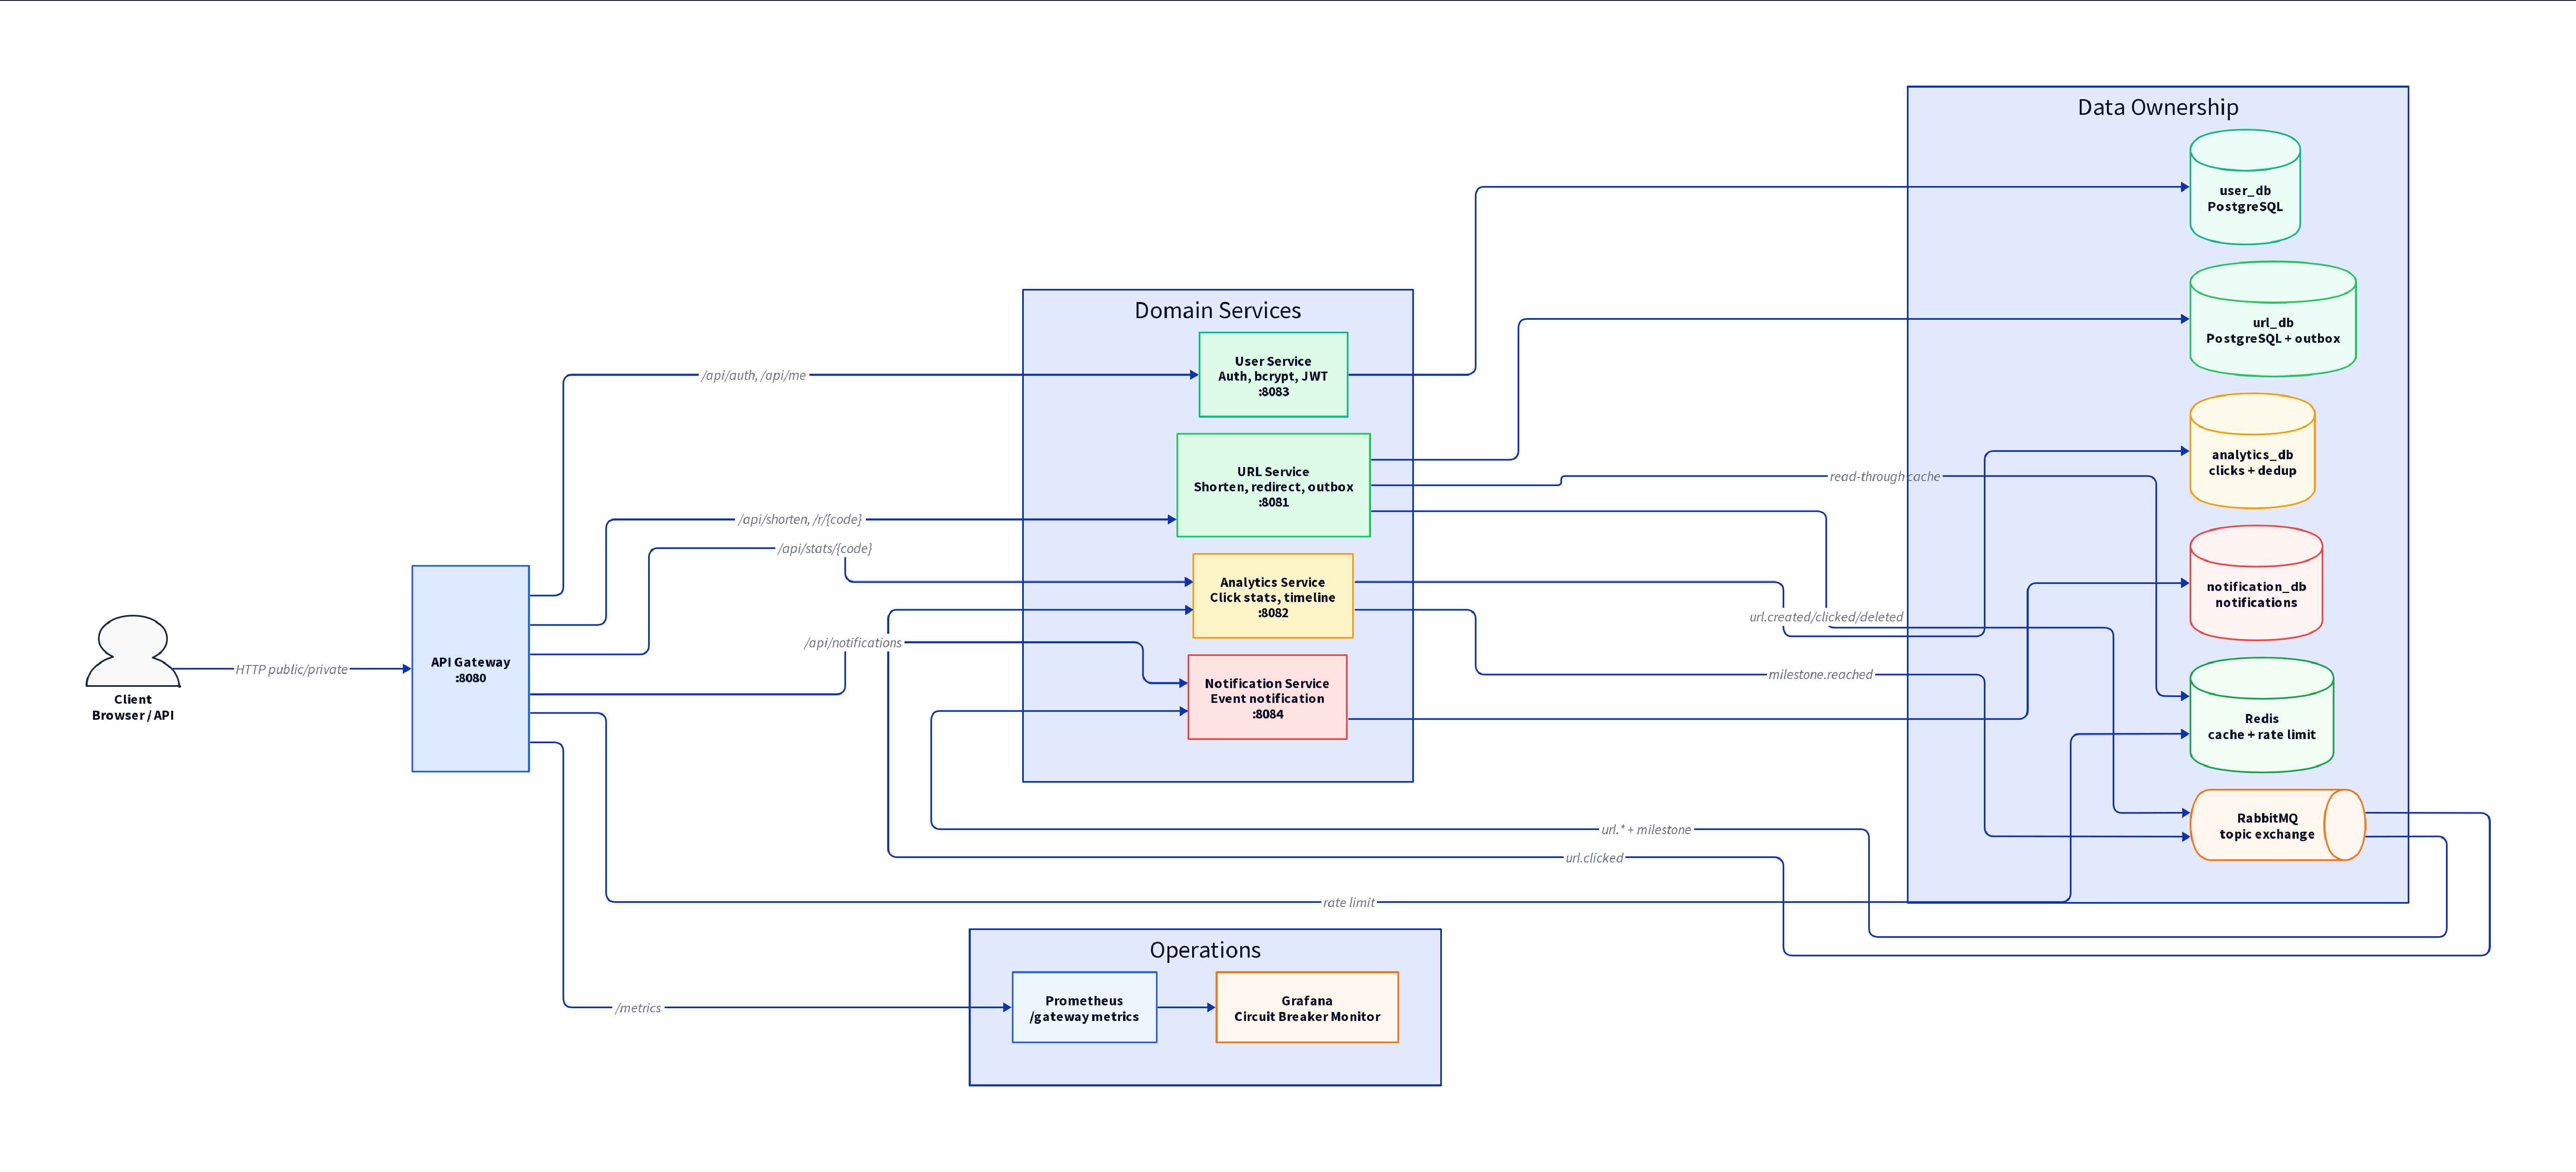
\includegraphics[width=0.92\textwidth,height=0.68\textheight,keepaspectratio]{architecture.pdf}
    \end{center}
    \vspace{-0.15cm}
    \begin{claimbox}{primary}
        \scriptsize Sơ đồ D2 này cố tình thể hiện cả runtime boundary, data ownership và operations để chứng minh đây là một hệ thống microservices có vận hành, không chỉ là nhiều package Go.
    \end{claimbox}
\end{frame}

\begin{frame}{Rubric SE361: mapping từng tiêu chí vào dự án}
    \scriptsize
    \begin{center}
    \begin{tabular}{>{\bfseries}p{0.24\textwidth}p{0.33\textwidth}p{0.33\textwidth}}
        \toprule
        Tiêu chí môn học & Hiện thực trong dự án & Slide/demo để bảo vệ \\
        \midrule
        DDD, SRP, Bounded Context & User, URL, Analytics, Notification, Gateway tách trách nhiệm rõ & Service responsibility + DB ownership \\
        RESTful API & Gateway expose endpoint public/private, service nội bộ HTTP/JSON & API surface, route table \\
        Async communication & RabbitMQ topic exchange, durable queue, event contract & Event pipeline D2 \\
        Database per Service & 4 PostgreSQL DB riêng, không shared schema & Database per service table \\
        Resilience & Rate limit, timeout, circuit breaker, fail-open Redis limiter & CB state machine + load test \\
        Observability & JSON logs, correlation ID, Prometheus, Grafana & Deployment/observability D2 \\
        Testing & Unit, smoke, e2e, k6 load test & Testing matrix \\
        \bottomrule
    \end{tabular}
    \end{center}
\end{frame}

\begin{frame}{Từ monolith sang microservices: quyết định thiết kế}
    \begin{columns}[T,onlytextwidth]
        \begin{column}{0.31\textwidth}
            \begin{claimbox}{danger}
                \centering\textbf{Monolith ngây thơ}\par\small
                Auth, shorten, redirect, analytics, notification cùng process và cùng DB. Dễ demo nhưng khó scale và dễ cascading failure.
            \end{claimbox}
        \end{column}
        \begin{column}{0.31\textwidth}
            \begin{claimbox}{accent}
                \centering\textbf{Tách service}\par\small
                Tách bounded context theo nghiệp vụ, service sở hữu schema riêng, chỉ giao tiếp qua API/event.
            \end{claimbox}
        \end{column}
        \begin{column}{0.31\textwidth}
            \begin{claimbox}{best}
                \centering\textbf{Vận hành được}\par\small
                Gateway bảo vệ edge, RabbitMQ hấp thụ side effect, Redis giảm tải hot path, Prometheus/Grafana quan sát lỗi.
            \end{claimbox}
        \end{column}
    \end{columns}
    \vspace{0.35cm}
    \begin{claimbox}{primary}
        \small \textbf{Luận điểm:} URL shortener là bài toán nhỏ nhưng có profile tải rất thực tế: redirect đọc nhiều, analytics ghi nhiều, notification là side effect; vì vậy microservices có lý do kỹ thuật, không phải tách cho có.
    \end{claimbox}
\end{frame}

\begin{frame}{Service Contract: User Service}
    \begin{columns}[T,onlytextwidth]
        \begin{column}{0.44\textwidth}
            \begin{claimbox}{secondary}
                \textbf{API}
                \begin{itemize}\scriptsize
                    \item \texttt{POST /register}: tạo user.
                    \item \texttt{POST /login}: phát JWT.
                    \item \texttt{GET /me}: đọc identity từ token.
                    \item \texttt{GET /health}: healthcheck container.
                \end{itemize}
            \end{claimbox}
        \end{column}
        \begin{column}{0.52\textwidth}
            \begin{claimbox}{primary}
                \textbf{Chi tiết đáng kể}
                \begin{itemize}\small
                    \item Email validate bằng regex và unique constraint.
                    \item Password tối thiểu 8 ký tự, hash bằng bcrypt.
                    \item JWT có issuer, issued-at, expiry, subject, email.
                    \item Body register/login giới hạn 1MB.
                    \item Có fake verify khi user không tồn tại để giảm timing leak.
                \end{itemize}
            \end{claimbox}
        \end{column}
    \end{columns}
\end{frame}

\begin{frame}{Service Contract: URL Service}
    \begin{columns}[T,onlytextwidth]
        \begin{column}{0.48\textwidth}
            \begin{claimbox}{best}
                \textbf{Domain commands}
                \begin{itemize}\small
                    \item Shorten URL: validate scheme, generate code, persist.
                    \item List URLs: cursor pagination, limit clamp 1..100.
                    \item Delete URL: ownership check, soft deactivate, cache invalidation.
                    \item Redirect: cache first, DB fallback, status 410 nếu expired/inactive.
                \end{itemize}
            \end{claimbox}
        \end{column}
        \begin{column}{0.48\textwidth}
            \begin{claimbox}{accent}
                \textbf{Domain events}
                \begin{itemize}\small
                    \item \texttt{url.created}: notification biết có link mới.
                    \item \texttt{url.clicked}: analytics ghi click.
                    \item \texttt{url.deleted}: notification biết link bị xóa.
                    \item Event ghi vào outbox cùng transaction với URL mutation.
                \end{itemize}
            \end{claimbox}
        \end{column}
    \end{columns}
\end{frame}

\begin{frame}{D2 Redirect Hot Path: nơi chịu tải cao nhất}
    \begin{center}
        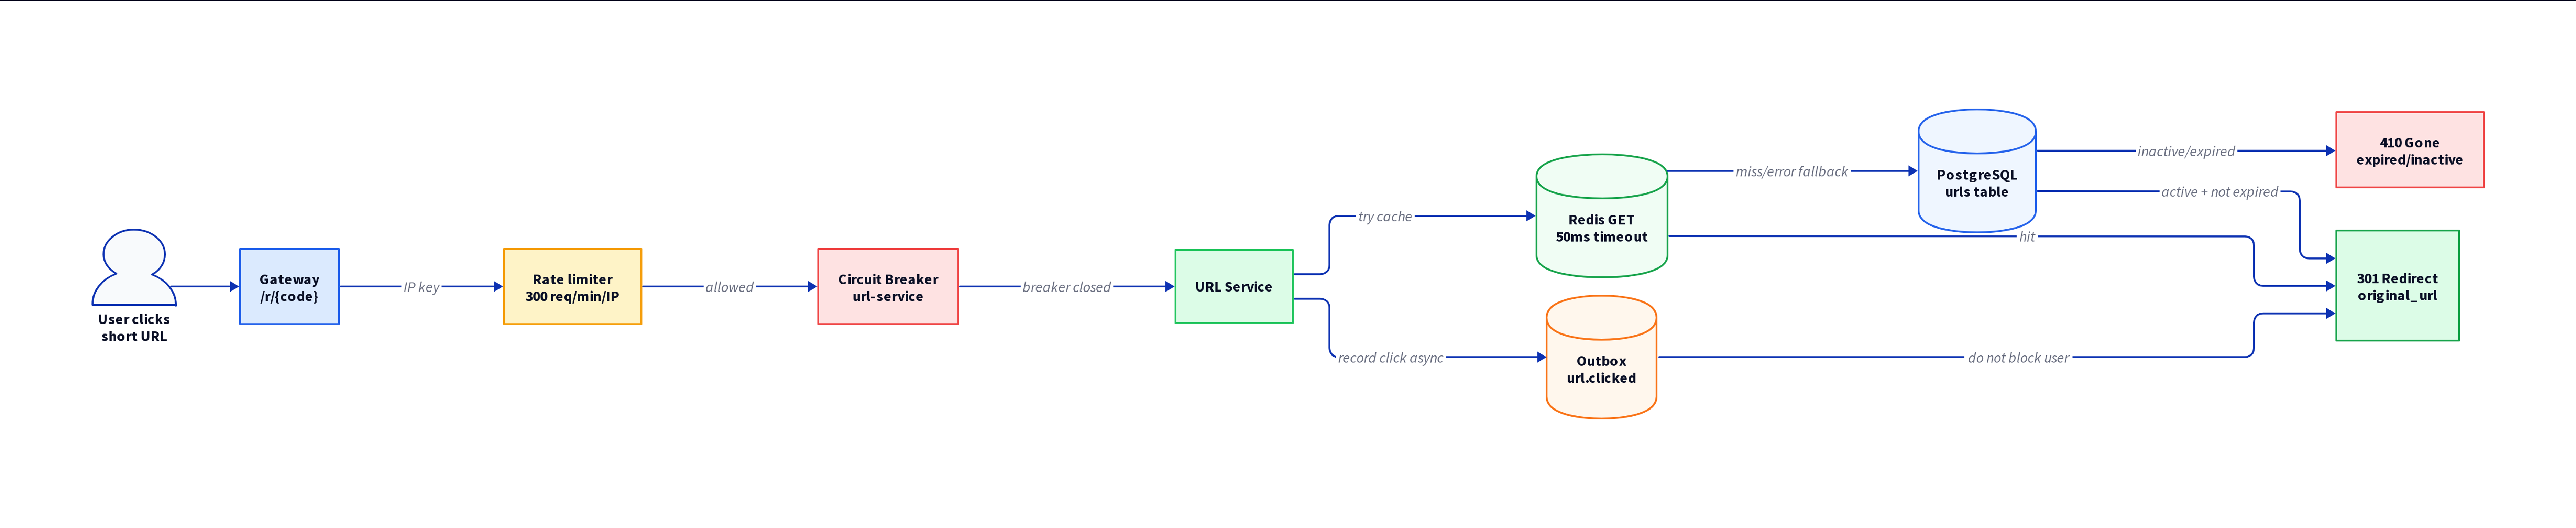
\includegraphics[width=0.95\textwidth,height=0.76\textheight,keepaspectratio]{redirect_flow.pdf}
    \end{center}
    \begin{claimbox}{best}
        \scriptsize Điểm cần nói khi demo: redirect không chờ analytics consumer. Click event được ghi async; người dùng nhận redirect nhanh nhất có thể.
    \end{claimbox}
\end{frame}

\begin{frame}{Short Code: nhỏ nhưng phải giải thích được}
    \begin{columns}[T,onlytextwidth]
        \begin{column}{0.49\textwidth}
            \begin{claimbox}{primary}
                \textbf{Thiết kế mã ngắn}
                \begin{itemize}\small
                    \item Alphabet base62: \texttt{a-zA-Z0-9}.
                    \item Độ dài 7 ký tự: \texttt{62\^{}7} $\approx$ 3.52 nghìn tỷ mã.
                    \item Sinh bằng \texttt{crypto/rand}, không dùng \texttt{math/rand}.
                    \item PostgreSQL unique constraint là hàng rào cuối.
                \end{itemize}
            \end{claimbox}
        \end{column}
        \begin{column}{0.47\textwidth}
            \begin{claimbox}{accent}
                \textbf{Collision handling}
                \begin{itemize}\small
                    \item Nếu insert đụng unique \texttt{short\_code}, service retry.
                    \item Retry tối đa 3 lần để tránh loop vô hạn.
                    \item Với 1 triệu URL, xác suất collision cực thấp theo dev docs.
                    \item Không cần coordination service để cấp mã trong scope đồ án.
                \end{itemize}
            \end{claimbox}
        \end{column}
    \end{columns}
\end{frame}

\begin{frame}{D2 Event Pipeline: Outbox + RabbitMQ + Consumers}
    \begin{center}
        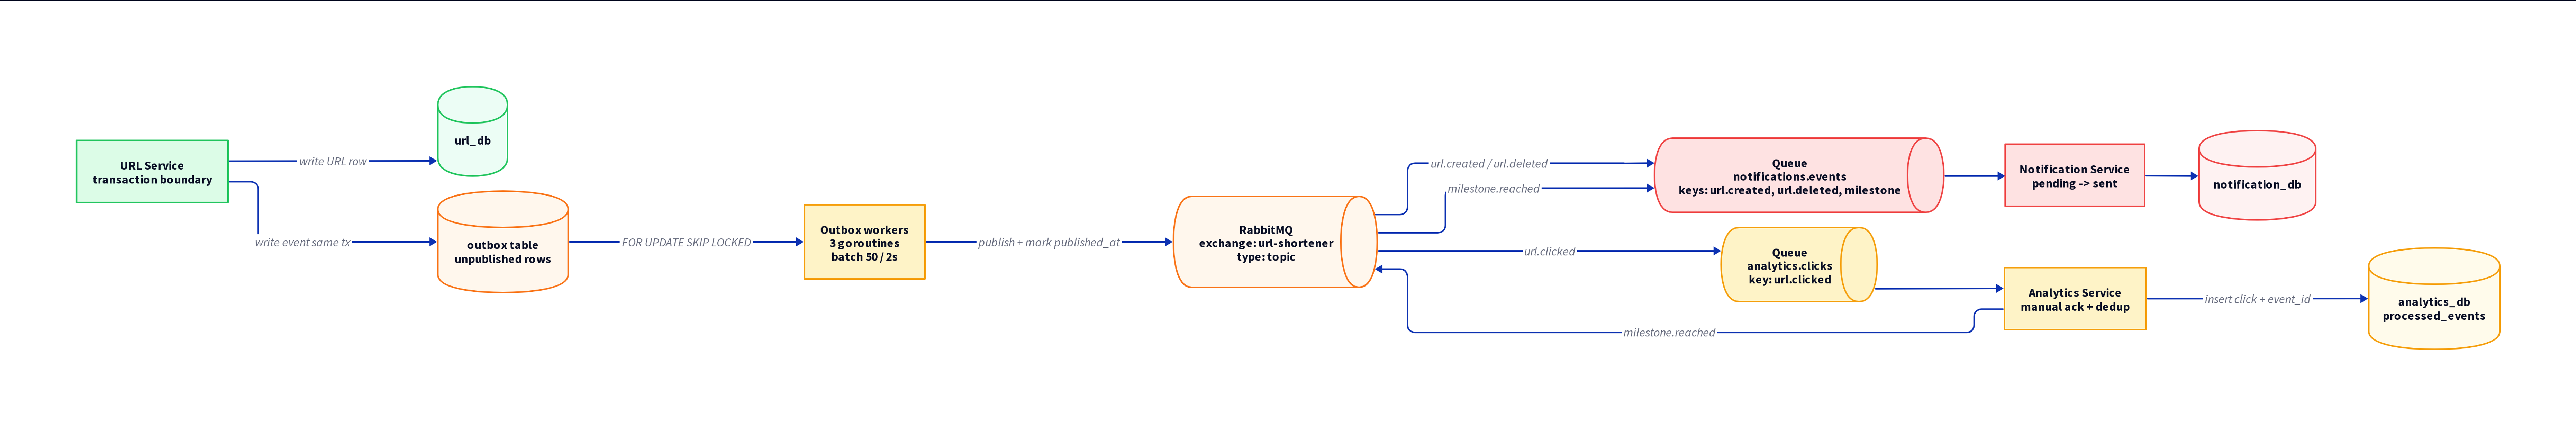
\includegraphics[width=0.95\textwidth,height=0.77\textheight,keepaspectratio]{event_pipeline.pdf}
    \end{center}
\end{frame}

\begin{frame}{RabbitMQ Topology: topic exchange có chủ đích}
    \begin{columns}[T,onlytextwidth]
        \begin{column}{0.46\textwidth}
            \begin{claimbox}{accent}
                \textbf{Exchange}
                \begin{itemize}\small
                    \item Name: \texttt{url-shortener}.
                    \item Type: \texttt{topic}.
                    \item Durable để queue/exchange sống qua restart.
                    \item Routing key mô tả domain event.
                \end{itemize}
            \end{claimbox}
        \end{column}
        \begin{column}{0.50\textwidth}
            \begin{claimbox}{primary}
                \textbf{Bindings}
                \begin{itemize}\small
                    \item \texttt{analytics.clicks} nhận \texttt{url.clicked}.
                    \item \texttt{notifications.events} nhận \texttt{url.created}, \texttt{url.deleted}, \texttt{milestone.reached}.
                    \item Analytics phát ngược \texttt{milestone.reached} khi đạt 10/100/1000 clicks.
                    \item Consumer không gọi chéo để hỏi thêm dữ liệu nếu event đã đủ payload.
                \end{itemize}
            \end{claimbox}
        \end{column}
    \end{columns}
\end{frame}

\begin{frame}{Data Consistency: chấp nhận eventual consistency có kiểm soát}
    \begin{columns}[T,onlytextwidth]
        \begin{column}{0.48\textwidth}
            \begin{claimbox}{danger}
                \textbf{Điều không làm}
                \begin{itemize}\small
                    \item Không distributed transaction 2PC.
                    \item Không shared DB để join trực tiếp.
                    \item Không hứa exactly-once toàn hệ thống.
                    \item Không để redirect gọi sync sang analytics/notification.
                \end{itemize}
            \end{claimbox}
        \end{column}
        \begin{column}{0.48\textwidth}
            \begin{claimbox}{best}
                \textbf{Điều đã làm}
                \begin{itemize}\small
                    \item Outbox đảm bảo DB mutation và event cùng transaction.
                    \item At-least-once delivery qua RabbitMQ.
                    \item Analytics dedup bằng \texttt{processed\_events}.
                    \item Milestone unique constraint tránh bắn nhiều lần.
                \end{itemize}
            \end{claimbox}
        \end{column}
    \end{columns}
\end{frame}

\begin{frame}{Schema Design: chi tiết để tránh bị hỏi hổng}
    \scriptsize
    \begin{center}
    \begin{tabular}{>{\bfseries}p{0.18\textwidth}p{0.34\textwidth}p{0.38\textwidth}}
        \toprule
        DB & Bảng chính & Lý do thiết kế \\
        \midrule
        \texttt{user\_db} & \texttt{users(id, email, password\_hash, created\_at)} & User service sở hữu identity; email unique để chống duplicate. \\
        \texttt{url\_db} & \texttt{urls}, \texttt{outbox} & URL là source of truth; outbox là cầu nối sang messaging. \\
        \texttt{analytics\_db} & \texttt{clicks}, \texttt{processed\_events}, \texttt{milestones} & Click append-only, event dedup, milestone unique. \\
        \texttt{notification\_db} & \texttt{notifications(user\_id, payload, status, sent\_at)} & Side effect được lưu trạng thái để debug/retry. \\
        \bottomrule
    \end{tabular}
    \end{center}
    \vspace{0.3cm}
    \begin{claimbox}{secondary}
        \small \textbf{Indexes cần nhắc:} \texttt{short\_code} cho redirect, \texttt{user\_id + created\_at} cho list URL, \texttt{outbox unpublished} cho worker, \texttt{processed\_events(event\_id)} cho dedup.
    \end{claimbox}
\end{frame}

\begin{frame}{Analytics: không chỉ đếm tổng click}
    \begin{columns}[T,onlytextwidth]
        \begin{column}{0.32\textwidth}
            \begin{claimbox}{primary}
                \centering\textbf{Counters}\par\small
                Total clicks, last 24h, last 7d. Các query chạy song song để giảm latency API stats.
            \end{claimbox}
        \end{column}
        \begin{column}{0.32\textwidth}
            \begin{claimbox}{accent}
                \centering\textbf{Breakdown}\par\small
                Top referers, timeline theo day/hour, lưu user-agent và referer từ click event.
            \end{claimbox}
        \end{column}
        \begin{column}{0.32\textwidth}
            \begin{claimbox}{best}
                \centering\textbf{Milestone}\par\small
                Khi đạt 10, 100, 1000 clicks, analytics phát \texttt{milestone.reached} cho notification.
            \end{claimbox}
        \end{column}
    \end{columns}
\end{frame}

\begin{frame}{D2 Deployment \& Observability: chạy được cả stack}
    \begin{center}
        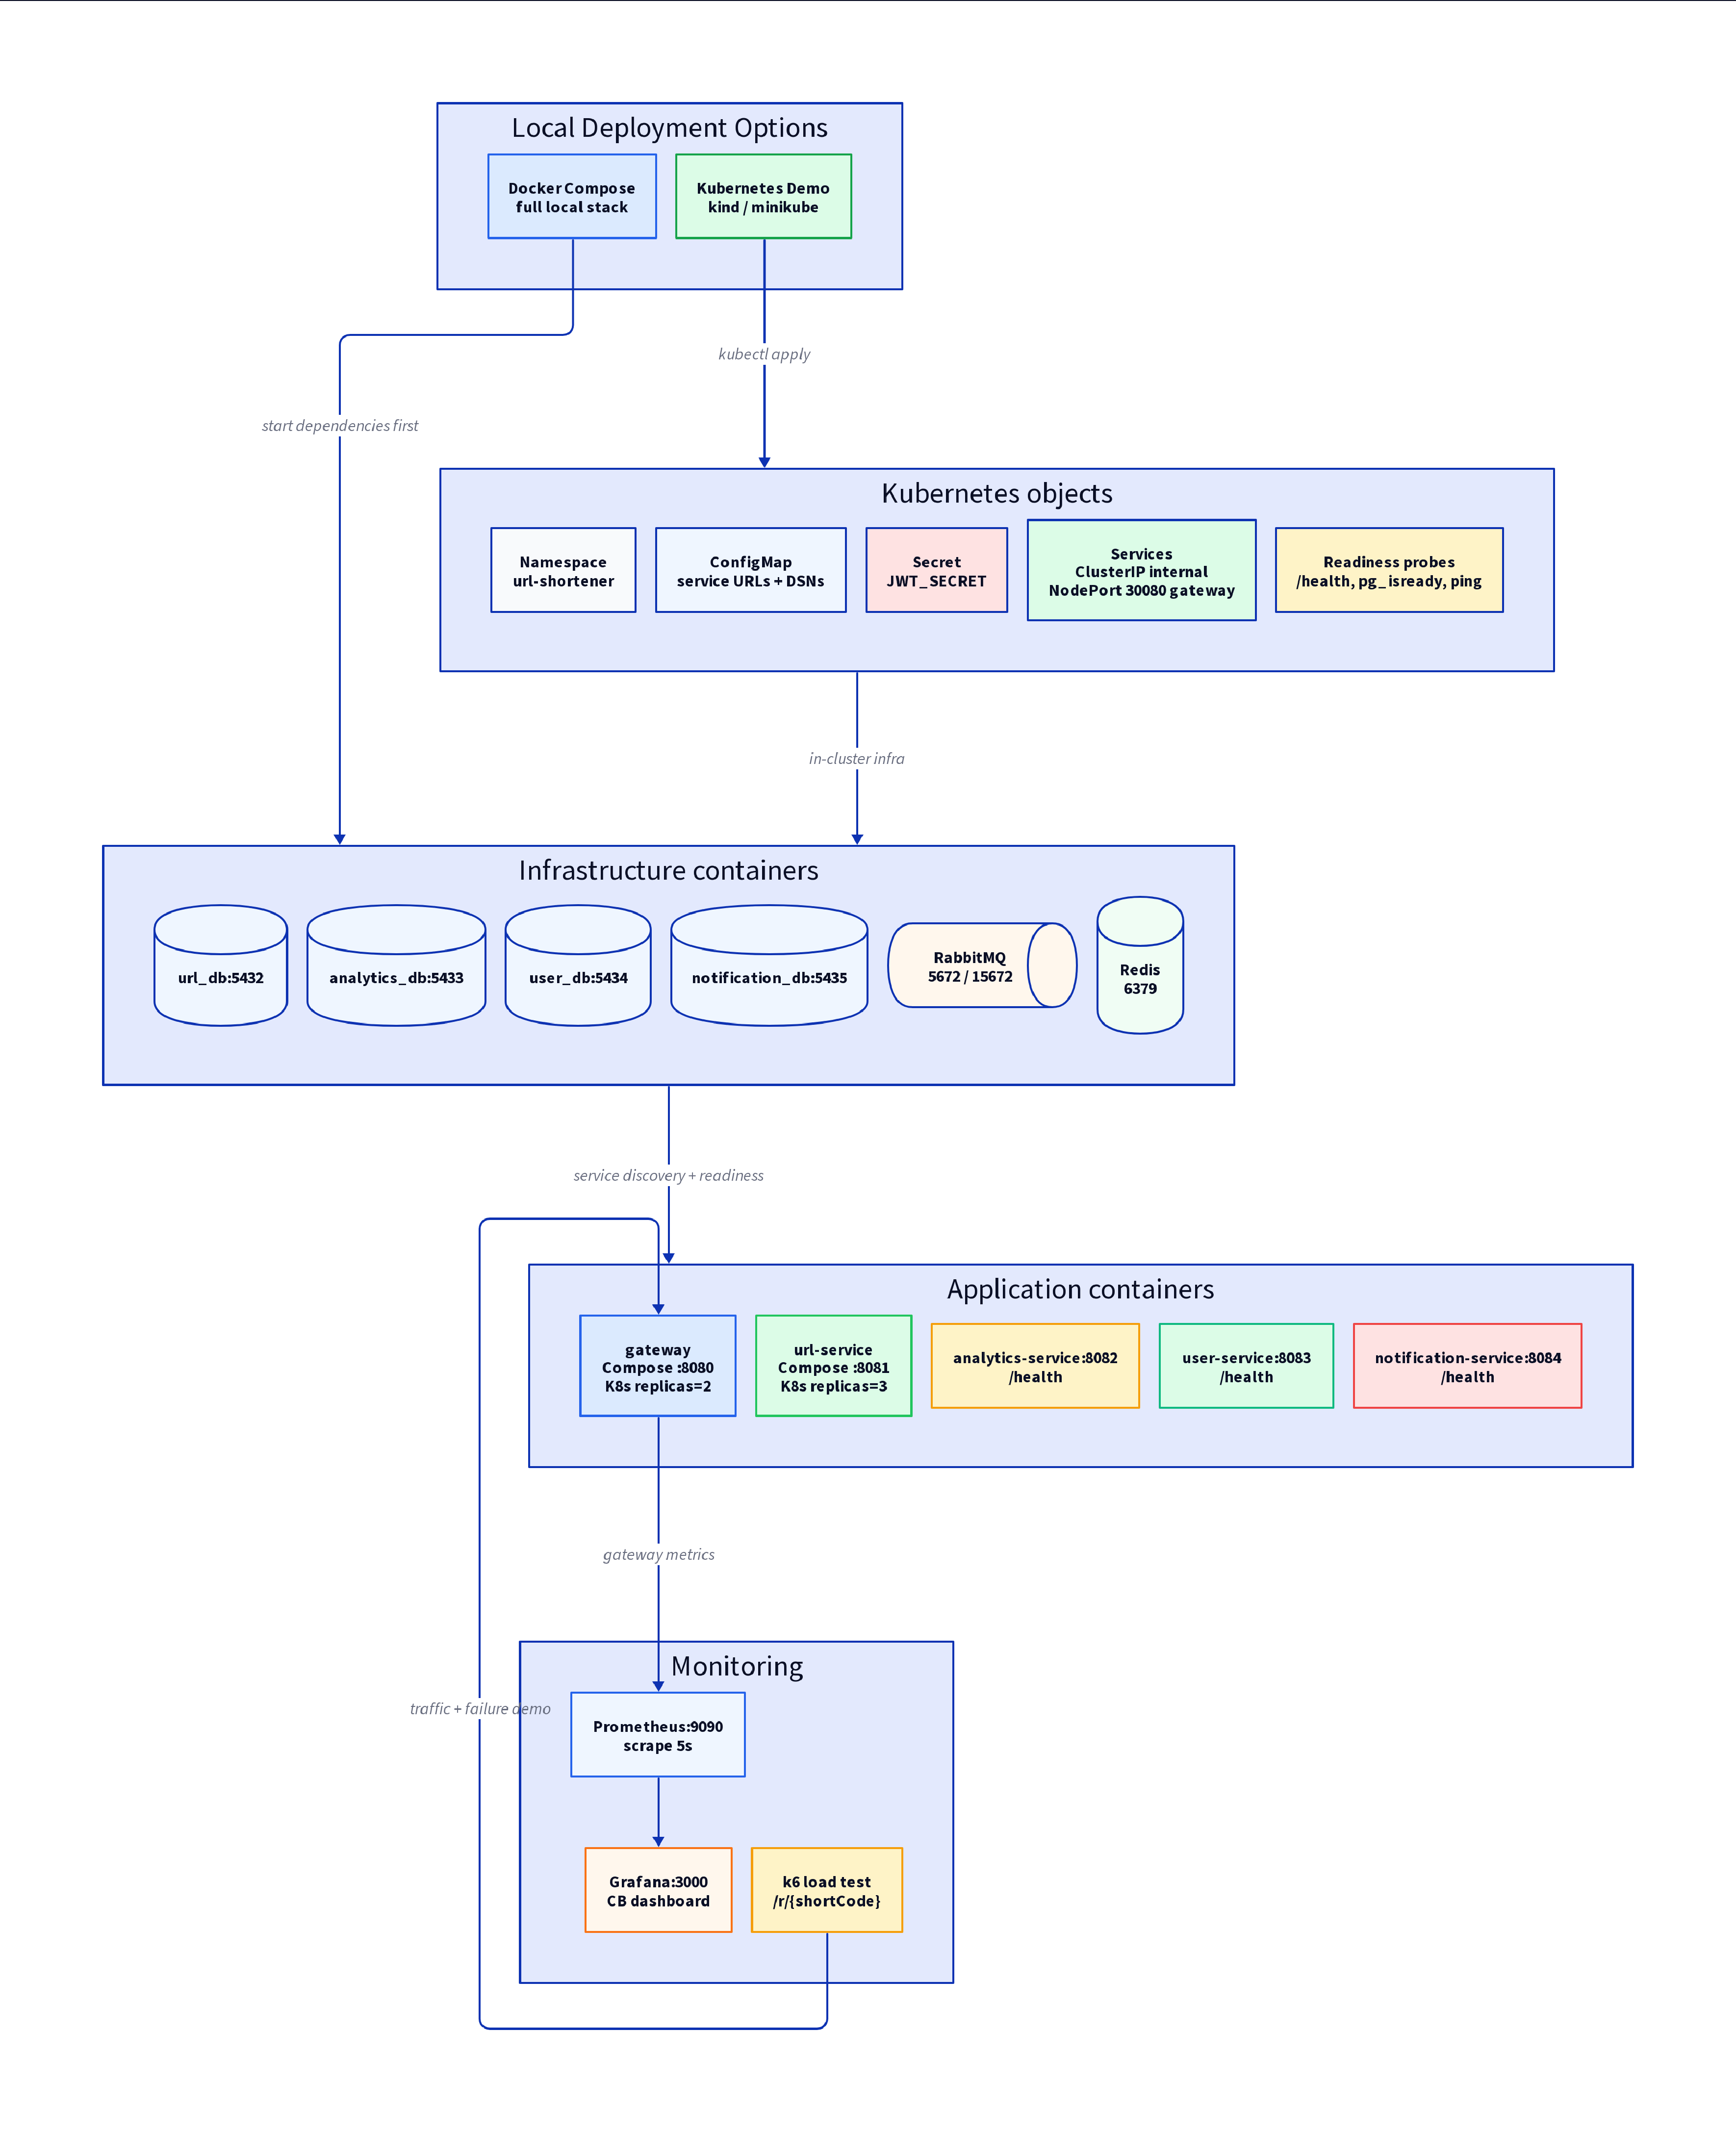
\includegraphics[width=0.95\textwidth,height=0.76\textheight,keepaspectratio]{deployment_observability.pdf}
    \end{center}
\end{frame}

\begin{frame}{Docker Compose: thứ tự khởi động và healthcheck}
    \begin{columns}[T,onlytextwidth]
        \begin{column}{0.48\textwidth}
            \begin{claimbox}{primary}
                \textbf{Infrastructure first}
                \begin{itemize}\small
                    \item 4 PostgreSQL containers có \texttt{pg\_isready}.
                    \item RabbitMQ dùng \texttt{rabbitmq-diagnostics ping}.
                    \item Redis dùng \texttt{redis-cli ping}.
                    \item Volumes riêng cho DB, RabbitMQ, Redis, Prometheus, Grafana.
                \end{itemize}
            \end{claimbox}
        \end{column}
        \begin{column}{0.48\textwidth}
            \begin{claimbox}{secondary}
                \textbf{App depends on healthy deps}
                \begin{itemize}\small
                    \item Service chỉ start khi DB/broker/cache healthy.
                    \item Mỗi app expose \texttt{/health}.
                    \item Gateway phụ thuộc 4 domain service healthy.
                    \item Smoke test kiểm tra ports 8080--8084.
                \end{itemize}
            \end{claimbox}
        \end{column}
    \end{columns}
\end{frame}

\begin{frame}{Prometheus metrics: không chỉ có log}
    \begin{columns}[T,onlytextwidth]
        \begin{column}{0.52\textwidth}
            \begin{claimbox}{primary}
                \textbf{Gateway metrics}
                \begin{itemize}\tiny
                    \item \texttt{gateway\_requests\_total}
                    \item \texttt{gateway\_request\_duration\_seconds}
                    \item \texttt{gateway\_circuit\_breaker\_state}
                    \item \texttt{gateway\_circuit\_breaker\_trips\_total}
                    \item \texttt{gateway\_circuit\_breaker\_rejected\_total}
                \end{itemize}
            \end{claimbox}
        \end{column}
        \begin{column}{0.44\textwidth}
            \begin{claimbox}{accent}
                \textbf{Grafana panels}
                \begin{itemize}\small
                    \item Circuit Breaker State: 0/1/2.
                    \item Requests/sec by status class.
                    \item Error Rate \%.
                    \item CB Trips total.
                \end{itemize}
            \end{claimbox}
        \end{column}
    \end{columns}
\end{frame}

\begin{frame}{Load Test Script: thuyết phục bằng quy trình demo}
    \begin{columns}[T,onlytextwidth]
        \begin{column}{0.47\textwidth}
            \begin{claimbox}{best}
                \textbf{Happy path}
                \begin{enumerate}\small
                    \item \texttt{docker compose up -d --build}
                    \item \texttt{./scripts/smoke\_test.sh}
                    \item \texttt{k6 run scripts/load\_test.js}
                    \item k6 register, login, shorten URL.
                    \item Traffic tập trung vào \texttt{/r/\{shortCode\}}.
                \end{enumerate}
            \end{claimbox}
        \end{column}
        \begin{column}{0.49\textwidth}
            \begin{claimbox}{danger}
                \textbf{Failure path}
                \begin{enumerate}\small
                    \item Đang load test thì stop \texttt{url-service}.
                    \item Gateway bắt đầu connection error.
                    \item Sau 5 lỗi trong 10s: breaker OPEN.
                    \item Request mới trả 503 nhanh, không chờ timeout downstream.
                    \item Start lại service, 30s sau HALF\_OPEN probe.
                \end{enumerate}
            \end{claimbox}
        \end{column}
    \end{columns}
\end{frame}

\begin{frame}{Security Threat Model ngắn}
    \scriptsize
    \begin{center}
    \begin{tabular}{>{\bfseries}p{0.22\textwidth}p{0.34\textwidth}p{0.34\textwidth}}
        \toprule
        Rủi ro & Cơ chế hiện tại & Hạn chế / mở rộng \\
        \midrule
        Password leak & bcrypt hash, không lưu plaintext & Cần secret rotation, password policy mạnh hơn \\
        JWT tampering & Verify HMAC signing method, issuer, expiry & Chưa có refresh/revocation \\
        URL abuse/spam & Rate limit theo IP, body limit auth & Có thể thêm per-user quota và CAPTCHA \\
        Privacy analytics & Hash IP trước khi lưu event & Salt config cần audit kỹ \\
        Unauthorized delete & Ownership check bằng user id & Có thể thêm RBAC/team ownership \\
        Secret exposure & Env config cho demo & Production cần Vault/K8s Secret \\
        \bottomrule
    \end{tabular}
    \end{center}
\end{frame}

\begin{frame}{Những câu hỏi khó và cách trả lời không bị hớ}
    \scriptsize
    \begin{center}
    \begin{tabular}{p{0.35\textwidth}p{0.55\textwidth}}
        \toprule
        Câu hỏi khó & Câu trả lời nên dùng \\
        \midrule
        Nếu RabbitMQ down lúc tạo URL? & URL và event vẫn nằm trong DB/outbox; worker publish lại khi broker phục hồi. \\
        Nếu consumer xử lý trùng event? & Analytics dedup bằng \texttt{processed\_events}; milestone có unique constraint. Notification duplicate là hạn chế đã nhận diện. \\
        Vì sao không Saga? & Use case không cần distributed transaction nhiều bước có compensation; Outbox + eventual consistency đủ phù hợp. \\
        Redis cache stale sau delete? & Delete URL set inactive trong DB và xóa cache Redis; DB vẫn là source of truth. \\
        Tại sao gateway verify JWT mà service vẫn cần biết user? & Gateway là lớp edge; downstream vẫn nhận identity qua header/context để enforce ownership. \\
        Có scale thật chưa? & Compose demo một replica; thiết kế stateless cho gateway/url-service và cache/event broker hỗ trợ scale ngang. \\
        \bottomrule
    \end{tabular}
    \end{center}
\end{frame}

\begin{frame}{Kết luận}
    \begin{center}
        \begin{claimbox}[width=0.84\textwidth, halign=center]{primary}
            \large \textbf{URL Shortener Microservices}\par
            \vspace{0.25cm}
            \small Một case study nhỏ nhưng đủ lát cắt của môn SE361: DDD, database-per-service, REST, messaging, event-driven, outbox, cache, JWT, rate limit, circuit breaker, monitoring, load testing và Docker deployment.
        \end{claimbox}
    \end{center}
    \vspace{0.35cm}
    \begin{columns}[T,onlytextwidth]
        \begin{column}{0.32\textwidth}\begin{claimbox}{secondary}\centering\textbf{Scalable}\par\small cache + async + stateless edge\end{claimbox}\end{column}
        \begin{column}{0.32\textwidth}\begin{claimbox}{accent}\centering\textbf{Resilient}\par\small rate limit + circuit breaker + outbox\end{claimbox}\end{column}
        \begin{column}{0.32\textwidth}\begin{claimbox}{best}\centering\textbf{Observable}\par\small logs + metrics + Grafana\end{claimbox}\end{column}
    \end{columns}
\end{frame}

\end{document}
